\documentclass{article}
\usepackage[utf8]{inputenc}
\usepackage[italian]{babel}
\usepackage{amsmath}
\usepackage{amssymb}
\usepackage{siunitx}
\usepackage{tabularray}
\usepackage{graphicx}
\usepackage{float}
% \usepackage{minted}
\usepackage[bottom]{footmisc}
\usepackage[page]{appendix}
\usepackage[mathscr]{euscript}
\newcommand*{\diam}{\varnothing}
\newcommand*{\best}[1]{{#1}_\text{best}}
\newcommand*{\bestp}[1]{{\left(#1\right)}_\text{best}}
\newcommand*{\pbest}[1]{\left({#1}_\text{best}\right)}
\newcommand*{\pbestp}[1]{\left({\left(#1\right)}_\text{best}\right)}
\newcommand*{\errrel}[1]{\frac{\delta #1}{{#1}_\text{best}}}
\title{
  Laboratorio di Fisica 1\\
  R11: Calorimetro ad azoto liquido
}
\author{Gruppo 15: Bergamaschi Riccardo, Graiani Elia, Moglia Simone}
\date{14/05/2024 – 21/05/2024}
\makeindex
\begin{document}

\maketitle

\begin{abstract}
  Mediante un calorimetro ad azoto liquido, il gruppo di lavoro
  ha misurato i calori specifici di quattro campioni;
  preliminarmente, è stato necessario determinare il
  calore latente di vaporizzazione dell'azoto.
\end{abstract}

\setcounter{section}{-1}
\section{Materiali e strumenti di misura utilizzati}
\begin{center}
\begin{tblr}{
  width=\textwidth,
  colspec={ X[2,m,j]X[1,m,c]X[1,m,c]X[1,m,c] },
  vlines,
}
  \hline
  \textbf{Strumento di misura} & \textbf{Soglia} & \textbf{Portata} & \textbf{Sensibilità} \\
  \hline
  Amperometro & $\qty{0.001}{A}$ & N./A. & $\qty{0.001}{A}$ \\
  \hline[dashed]
  Voltmetro & $\qty{0.01}{V}$ & N./A. & $\qty{0.01}{V}$ \\
  \hline[dashed]
  Cronometro & $\qty{0.01}{s}$ & $\qty{99.99}{s}$ & $\qty{0.01}{s}$ \\
  \hline[dashed]
  Bilancia di precisione & $\qty{0.01}{g}$ & $\qty{4000.00}{g}$ & $\qty{0.01}{g}$ \\
  \hline
\end{tblr}
\begin{tblr}{
  width=\textwidth,
  colspec={ X[m,j]X[3,m,j] },
  vlines,
}
  \hline
  \textbf{Altro} & \textbf{Descrizione/Note} \\
  \hline
  Calorimetro & {
    Quasi adiabatico,
    dotato di un tappo con un foro centrale per potervi immergere
    i materiali e permettere la fuoriuscita dell'azoto gassoso.
  } \\
  \hline[dashed]
  Azoto liquido & Contenuto nel calorimetro \\
  \hline[dashed]
  Resistenza & {
    Fissata all'interno del tappo, fornisce calore all'azoto liquido.
  } \\
  \hline[dashed]
  Videocamera & {
    Utilizzata per acquisire i dati mostrati dal
    cronometro e della bilancia di precisione
    contemporaneamente.
  } \\
  \hline[dashed]
  Generatore & {
    Fornisce corrente elettrica al circuito, composto dall'amperometro
    (collegato in serie) e da voltmetro e resistenza (collegati in
    parallelo).
  } \\
  \hline[dashed]
  Quattro campioni metallici & { Li chiameremo $\Xi,\Delta,\aleph,\nabla$. } \\
  \hline
\end{tblr}
\end{center}

\pagebreak


\section{Misurazione del calore latente di vaporizzazione dell'azoto}

\subsection{Esperienza e procedimento di misura}

\begin{enumerate}
  \item
    Posto il calorimetro sopra alla bilancia di precisione, avviamo
    l'acquisizione del filmato.
  \item
    Dopo almeno una decina di secondi, accendiamo il generatore
    in modo da fornire calore all'azoto per mezzo della resistenza.
  \item
    Passato circa un minuto, spegniamo il generatore per interrompere
    lo scambio di calore e
    dopo almeno un'altra decina di secondi terminiamo la registrazione
    del filmato.
  \item
    Ripetiamo lo stesso procedimento, ma inserendo un tappo in plastica
    nel foro centrale del tappo del calorimetro, in modo da evitare la
    fuoriuscita di azoto gassoso.
\end{enumerate}

\subsection{Analisi dei dati raccolti e conclusioni}
  Essendo l'azoto a temperatura di ebollizione, possiamo esprimere la
  quantità di calore assorbito ($\delta Q$) in un intervallo di tempo
  $\Delta t$ in funzione della massa di azoto evaporata ($-\Delta m$):
  \[\delta Q = - \lambda_\text{vap} \Delta m\] dove la costante
  $\lambda_\text{vap}$ è detta “calore latente di vaporizzazione”.

  Tuttavia, possiamo assumere che $\delta Q$ sia pari al calore sviluppato
  dalla resistenza per effetto Joule. Assumendo le dispersioni di energia
  trascurabili, vale:
  \[ \delta Q = \mathscr{P}\cdot\Delta t = i\cdot\Delta V\cdot\Delta t\]

  Si avrà allora:
  \[
    \lambda_{vap} = \frac{i\cdot\Delta V\cdot\Delta t}{-\Delta m}
      = \frac{i\cdot\Delta V}{-\gamma}
    \qquad \text{con} \quad
    \gamma = \frac{\Delta m}{\Delta t}.
  \]

  Grazie al filmato possiamo graficare la variazione della massa in funzione del tempo
  e, successivamente, costruire tre distinte rette di regressione.
  %TODO: inserire i grafici

\section{Misurazione dei calori specifici dei campioni}

\subsection{Esperienza e procedimento di misura}

Per ogni campione:
\begin{enumerate}
  \item
    Come prima, avviamo la cattura del filmato dopo aver posizionato il calorimetro
    sopra alla bilancia di precisione.
  \item
    Dopo circa una decina di secondi, lo inseriamo nel calorimetro, che poi andiamo
    a chiudere tramite un tappo in plastica.
  \item
    Passati uno o due minuti per assicurarci che lo scambio di calore tra azoto e campione
    sia terminato, possiamo rimuovere il pesetto dal calorimetro e, successivamente,
    interrompere la registrazione.
    
\end{enumerate}

\subsection{Analisi dei dati raccolti e conclusioni}



\begin{center}
  \begin{tblr}{ |c|c|c|c|c| }
    \hline
    Oggetto & $L\;\;(\unit{cm})$ & $\diam\;\;(\unit{mm})$ & $m\;\;(\unit{g})$ & $I_\text{CM}\;\;(10^{-5}\,\unit{kg\,m^2})$ \\
    \hline
    Asta & $60.0\pm0.1$ & $5.94\pm0.01$ & $45.82\pm0.01$ & $568.5\pm1.5$ \\
    \hline[dashed]
    Rotore & N./A. & $13.41\pm0.01$ & $22.4\pm0.1^*$ & $0.058\pm0.001^*$ \\
    \hline
  \end{tblr}
\end{center}\begin{center}
  \begin{tblr}{ |c|c|c|c|c|c| }
    \hline
    $i$ & $m_i\;\;(\unit{g})$ & $d_i^\text{\,ext}\;\;(\unit{mm})$ & $d_i^\text{\,int}\;\;(\unit{mm})$ & $h_i\;\;(\unit{mm})$ & $I_{\text{CM},i}\;(\unit{mg\,m^2})$ \\
    \hline
    A & $115.95\pm0.01$ & $29.95 \pm 0.05$ & $6.20 \pm 0.05$ & $19.93 \pm 0.01$ & $10.62\pm0.03$ \\
    \hline[dashed]
    B & $115.86\pm0.01$ & $29.95 \pm 0.05$ & $6.20 \pm 0.05$ & $19.89 \pm 0.01$ & $10.59\pm0.03$\\
    \hline[dashed]
    C & $71.46\pm0.01$ & $29.95 \pm 0.05$ & $6.20 \pm 0.05$ & $12.08 \pm 0.01$ & $5.047\pm0.018$\\
    \hline
  \end{tblr}
\end{center}

\emph{$[^*]$ Valori dati}

\pagebreak
%\subsubsection{La misura di $T$}
Il periodo dell'oscillazione è stato misurato individuando $N+1$ zeri
consecutivi di $\theta(t)$, diciamo $\left\{t_0,t_1,\dots,t_N\right\}$.
Allora, poiché tra uno zero e l'altro corre metà periodo, è possibile
calcolare $T$ in questo modo: $T = \frac{2}{N}(t_N - t_0)$

Il gruppo di lavoro ha scelto $N$ di volta in volta, in modo tale che
fosse proporzionale al numero di oscillazioni compiute dal pendolo
prima di fermarsi. Complessivamente, $N$ ha assunto valori da $30$ a
$180$.

\vspace{2mm}
%\subsubsection{Il calcolo di $g$}

Come descritto sopra, il gruppo di lavoro ha calcolato, per ogni
configurazione $\Gamma$,
i valori di $\frac{I_z^\text{tot}}{Mr_\text{CM}}$
e $\frac{T^2}{4\pi^2}$, riportati nel grafico seguente.

Come è possibile osservare dalla relazione che le lega, la dipendenza
tra queste due grandezze è lineare: questo ci permette di determinare
il valore di $g$ come coefficiente angolare di una retta di regressione.

\begin{center}
\begin{figure}[H]
  %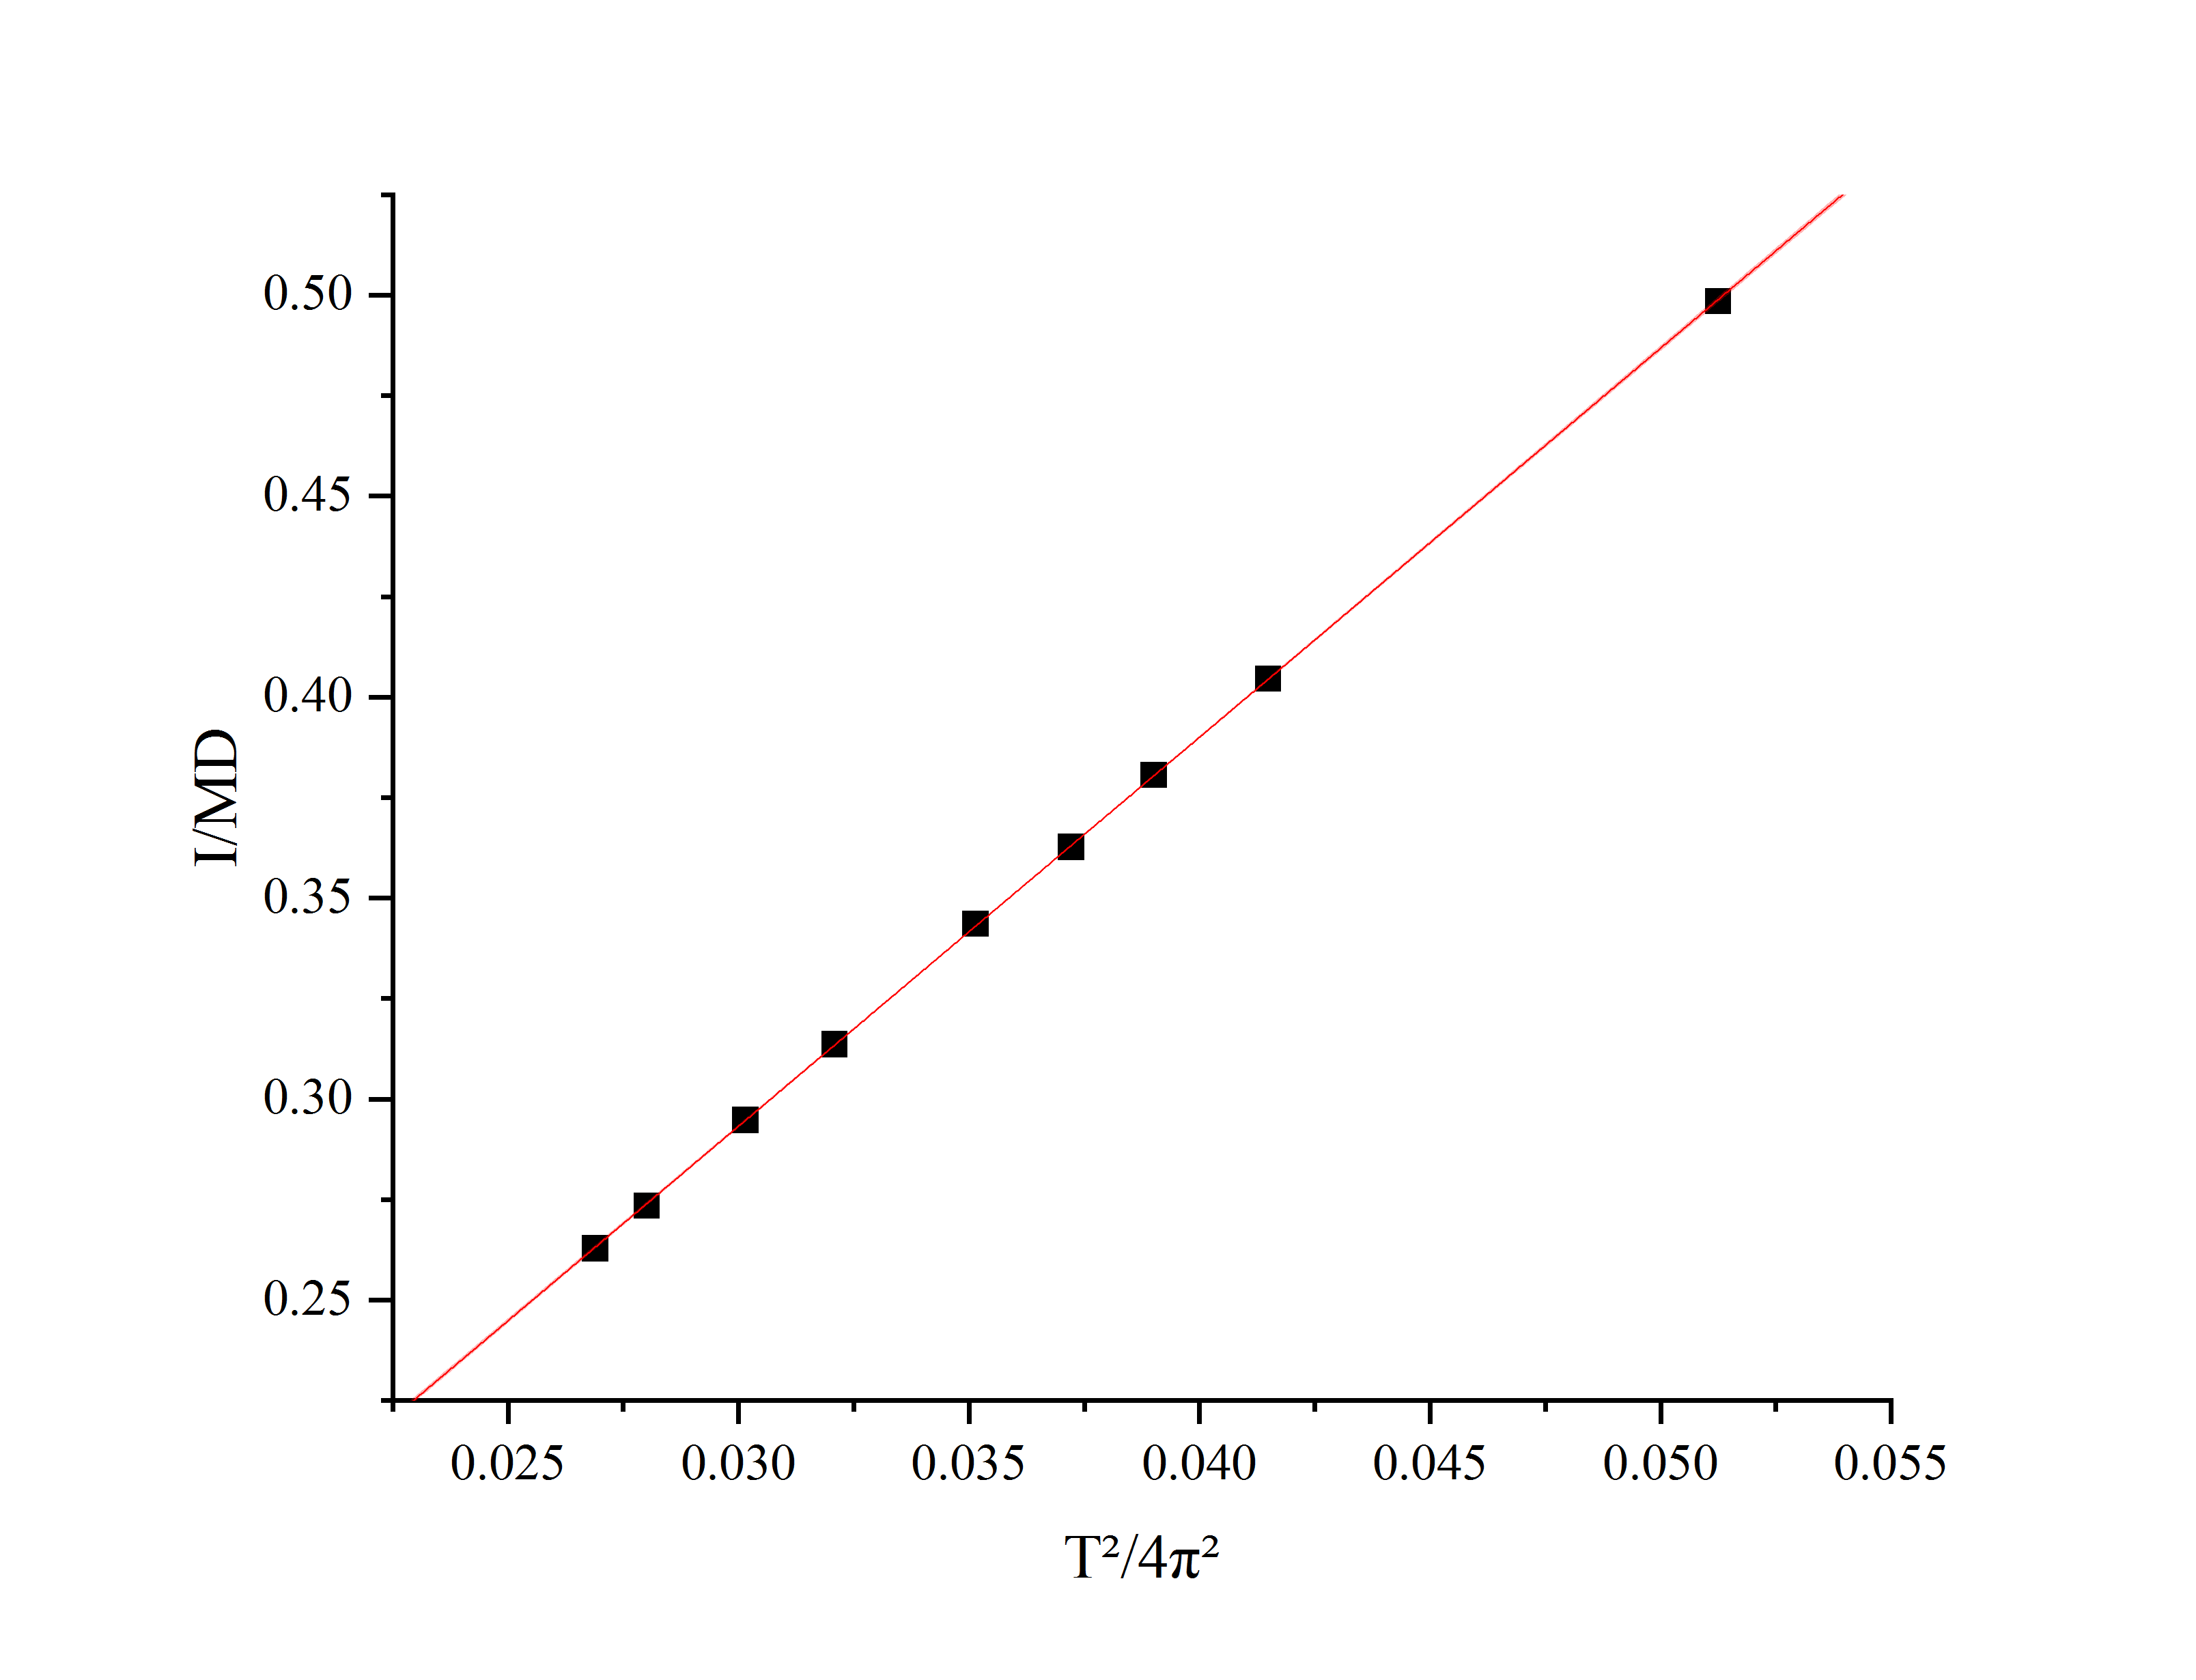
\includegraphics[trim={2cm 1cm 2cm 2.1cm},clip,width=\textwidth]{img/regressione.png}
  \caption[]{\emph{
    In rosso, la retta di regressione lineare e in rosa,
    appena visibile, la sua regione di incertezza.
    (le barre di errore sull'ascissa sono così ridotte
    da risultare invisibili)
  }}
\end{figure}
\end{center}

\begin{itemize}
  \item Intercetta $= (0.003 \pm 0.005)\;\unit{m}$
  \item Coefficiente angolare $g = (9.68 \pm 0.13)\;\unit{m\per s^2}$
\end{itemize}
\pagebreak
I risultati della regressione lineare sono chiaramente compatibili
con i valori attesi. Infatti:
\begin{itemize}
  \item Secondo il modello fisico utilizzato, l'intercetta dovrebbe
  essere nulla; in effetti, $(0.003\pm0.005)\;\unit{m}$ è compatibile
  con $\qty{0}{m}$.
  \item Il valore di $g$ atteso è $\qty{9.806}{m\per s^2}$; si può
  osservare facilmente che il valore misurato,
  $(9.68\pm0.13)\;\unit{m \per s^2}$, è compatibile con esso.
\end{itemize}

Possiamo pertanto concludere che l'esperienza ha avuto successo:
mediante l'apparato sperimentale abbiamo ottenuto una misura di $g$
compatibile con quella attesa.

\pagebreak
\subsection{Misura dello smorzamento}

\emph{
  In questa sezione, illustreremo come il gruppo di lavoro abbia
  valutato lo smorzamento del moto e quanto questo sia significativo,
  prendendo come esempio la configurazione $\Gamma=\left\{\right\}$,
  dove il pendolo fisico è composto solamente da asta e rotore, senza
  l'aggiunta di cilindri.
}

\emph{
  Il gruppo di lavoro ha effettuato gli stessi passaggi per tutte le
  altre configurazioni: i risultati saranno messi in evidenza alla
  fine della sezione.
}
\vspace{2mm}

Sempre applicando la seconda equazione cardinale della dinamica,
è facile ricavare l'equazione differenziale che caratterizza il moto
del sistema sotto l'effetto delle forze di attrito.
Approssimando, come prima, $\sin(\theta)\simeq\theta$, si ottiene:
\[ \ddot{\theta} = -2\lambda\dot{\theta} -\frac{Mg\,r_\text{CM}}{I_z^\text{\,tot}} \theta \]

dove $\lambda$ è una costante legata allo smorzamento del moto.
Le soluzioni di questa equazione differenziale sono infatti della forma:
\[\theta(t) = \theta_0\cos(\omega t)\,e^{-\lambda t}\]

dove la pulsazione del moto, $\omega$, è data da:
\[
  \omega^2 = \omega_0^2 - \lambda^2
  \qquad\text{con}\qquad
  \omega_0 = \sqrt{\frac{Mg\,r_\text{CM}}{I_z^\text{\,tot}}}.
\]

\begin{center}
  \begin{figure}[H]
    % trim={< v > ^}
    %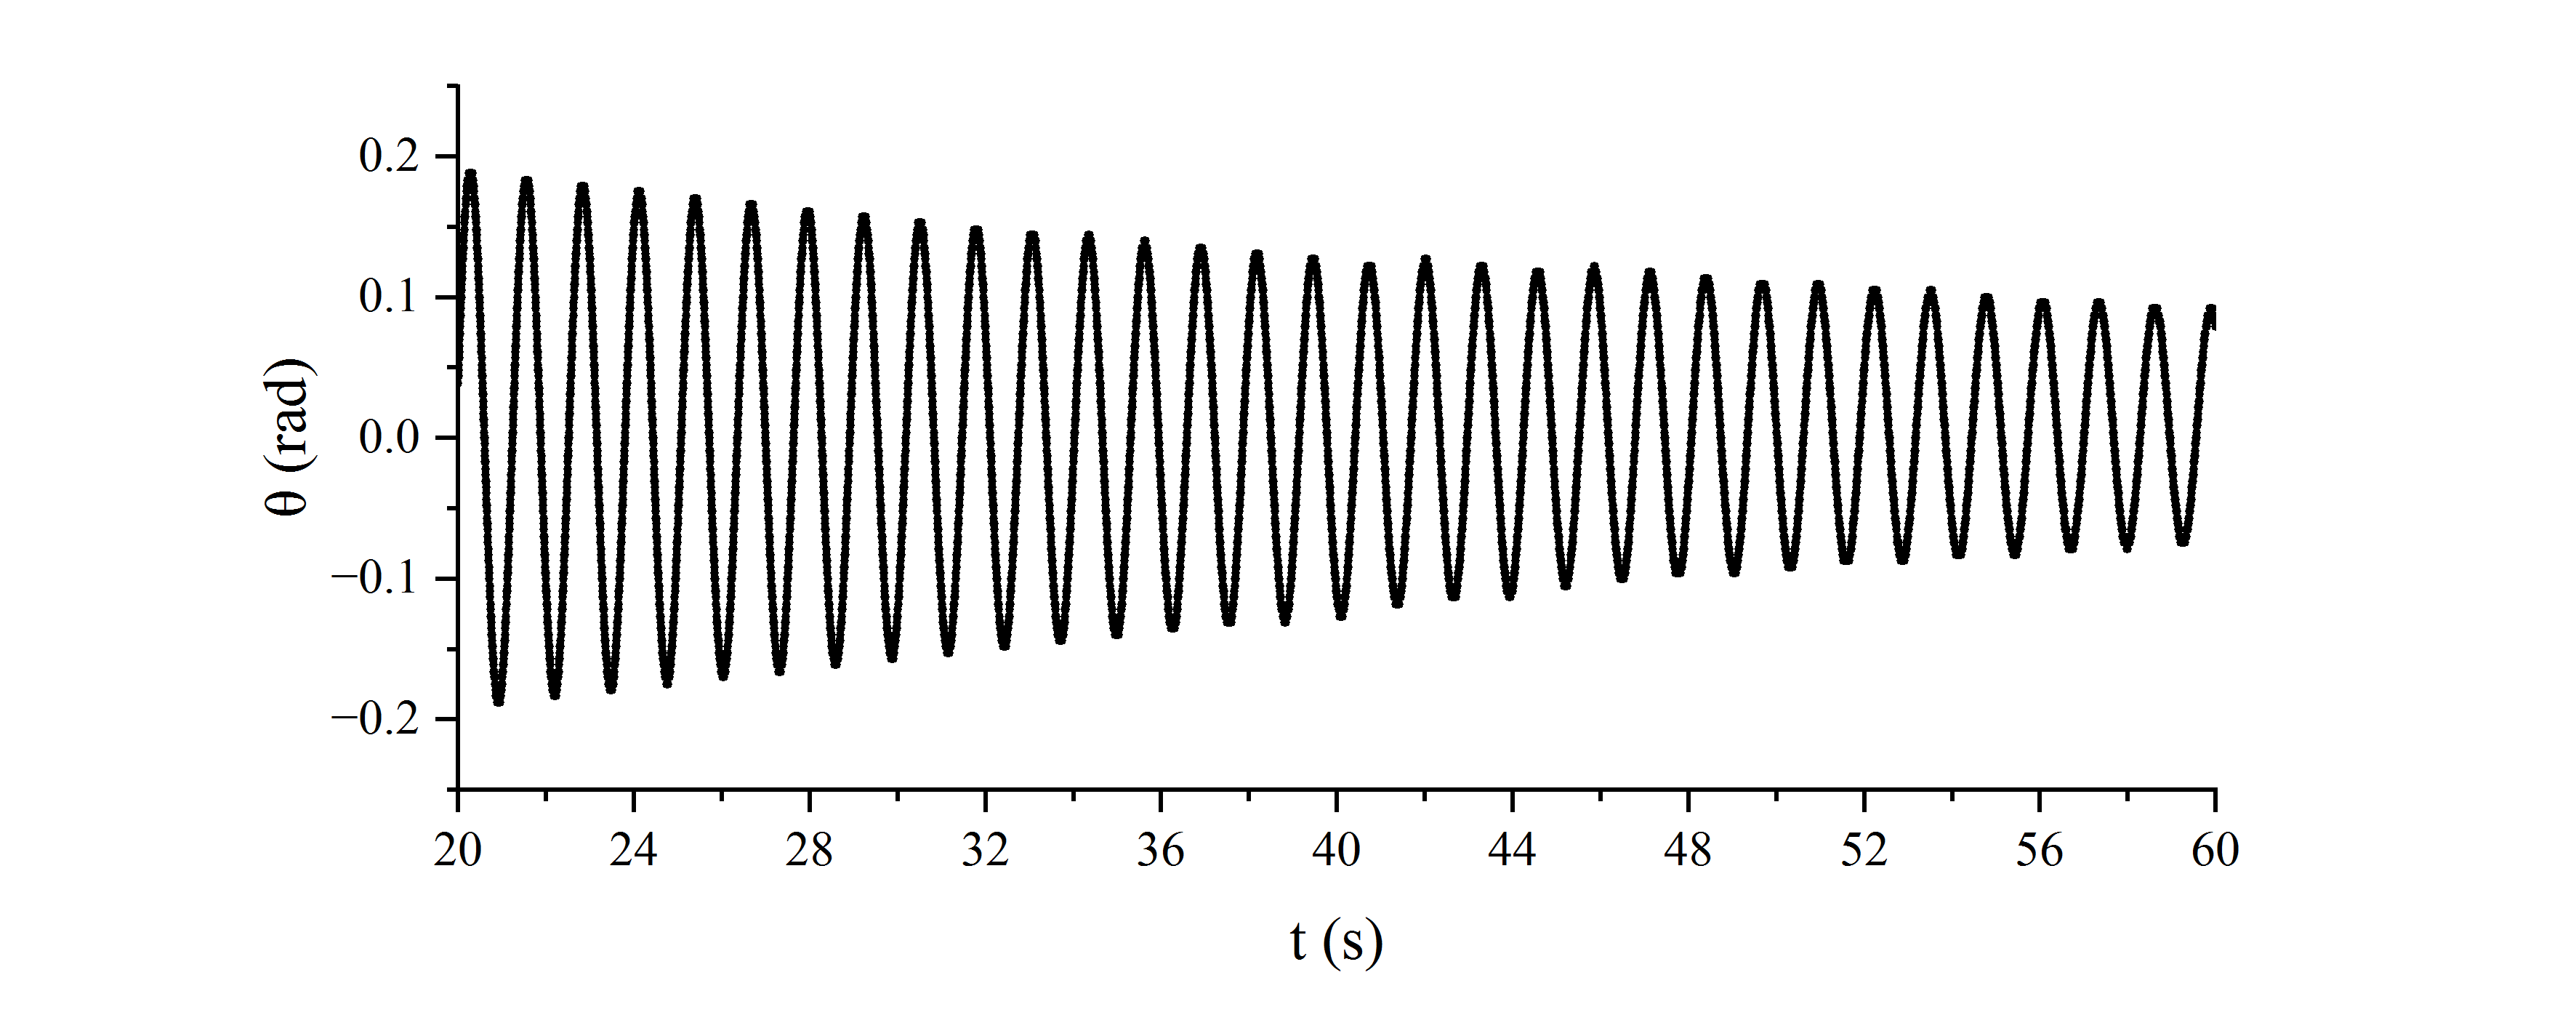
\includegraphics[trim={2cm .5cm 2cm .5cm},clip,width=\textwidth]{img/Graph1.png}
    \caption[]{\emph{
      Parte dei dati di un'acquisizione di $\theta(t)$
      con $\Gamma=\left\{\right\}$,
      come raccolti dal sensore di rotazione,
      riportati su una larga scala temporale.
      Si può chiaramente notare lo smorzamento
      del moto.
    }}
  \end{figure}
\end{center}

Per stimare $\lambda$, il gruppo di lavoro ha proceduto come segue:
\begin{enumerate}
  \item
    Per prima cosa, abbiamo individuato i massimi dei nostri dati,
    ovvero gli insiemi di punti della forma
    $\left\{t_i,t_{i+1},\dots,t_j\right\}\times\left\{\theta_k\right\}$
    tali che $\theta(t_{i-1}) < \theta_k > \theta(t_{j+1})$.
  \item
    Per ogni massimo, ne abbiamo calcolato il punto medio,
    prendendo come $\delta t_\text{picco}$ la semidispersione $\frac{1}{2}(t_j - t_i) + \delta t$.
  \item
    Infine, abbiamo graficato i punti così trovati
    su scala logaritmica e
    abbiamo effettuato una regressione lineare (pesata\footnote{
      $\delta\!\ln{\left|\theta\right|}$, infatti, varia molto,
      nonostante $\delta\!\left|\theta\right|$ sia costante:
      ciò è conseguenza della propagazione degli errori.
      È inoltre possibile osservarlo nella \emph{Figura 2}.
    })
    sulle nuove ordinate. Il coefficiente angolare di tale
    regressione dovrebbe essere proprio $-\lambda$.
  \item
    Abbiamo ripetuto i tre punti precedenti sugli stessi dati,
    con $\theta$ cambiato di segno: così facendo, ai massimi
    si sostituiscono i minimi e tutto il resto dell'analisi
    è analoga. Per ogni configurazione abbiamo pertanto ottenuto
    due diversi valori di $\lambda$: $\lambda_\text{min}$ e
    $\lambda_\text{max}$. Abbiamo scelto di porre
    $\lambda=\frac{1}{2}(\lambda_\text{min}+\lambda_\text{max})$.
\end{enumerate}

\begin{center}
  \begin{figure}[H]
    % trim={< v > ^}
    %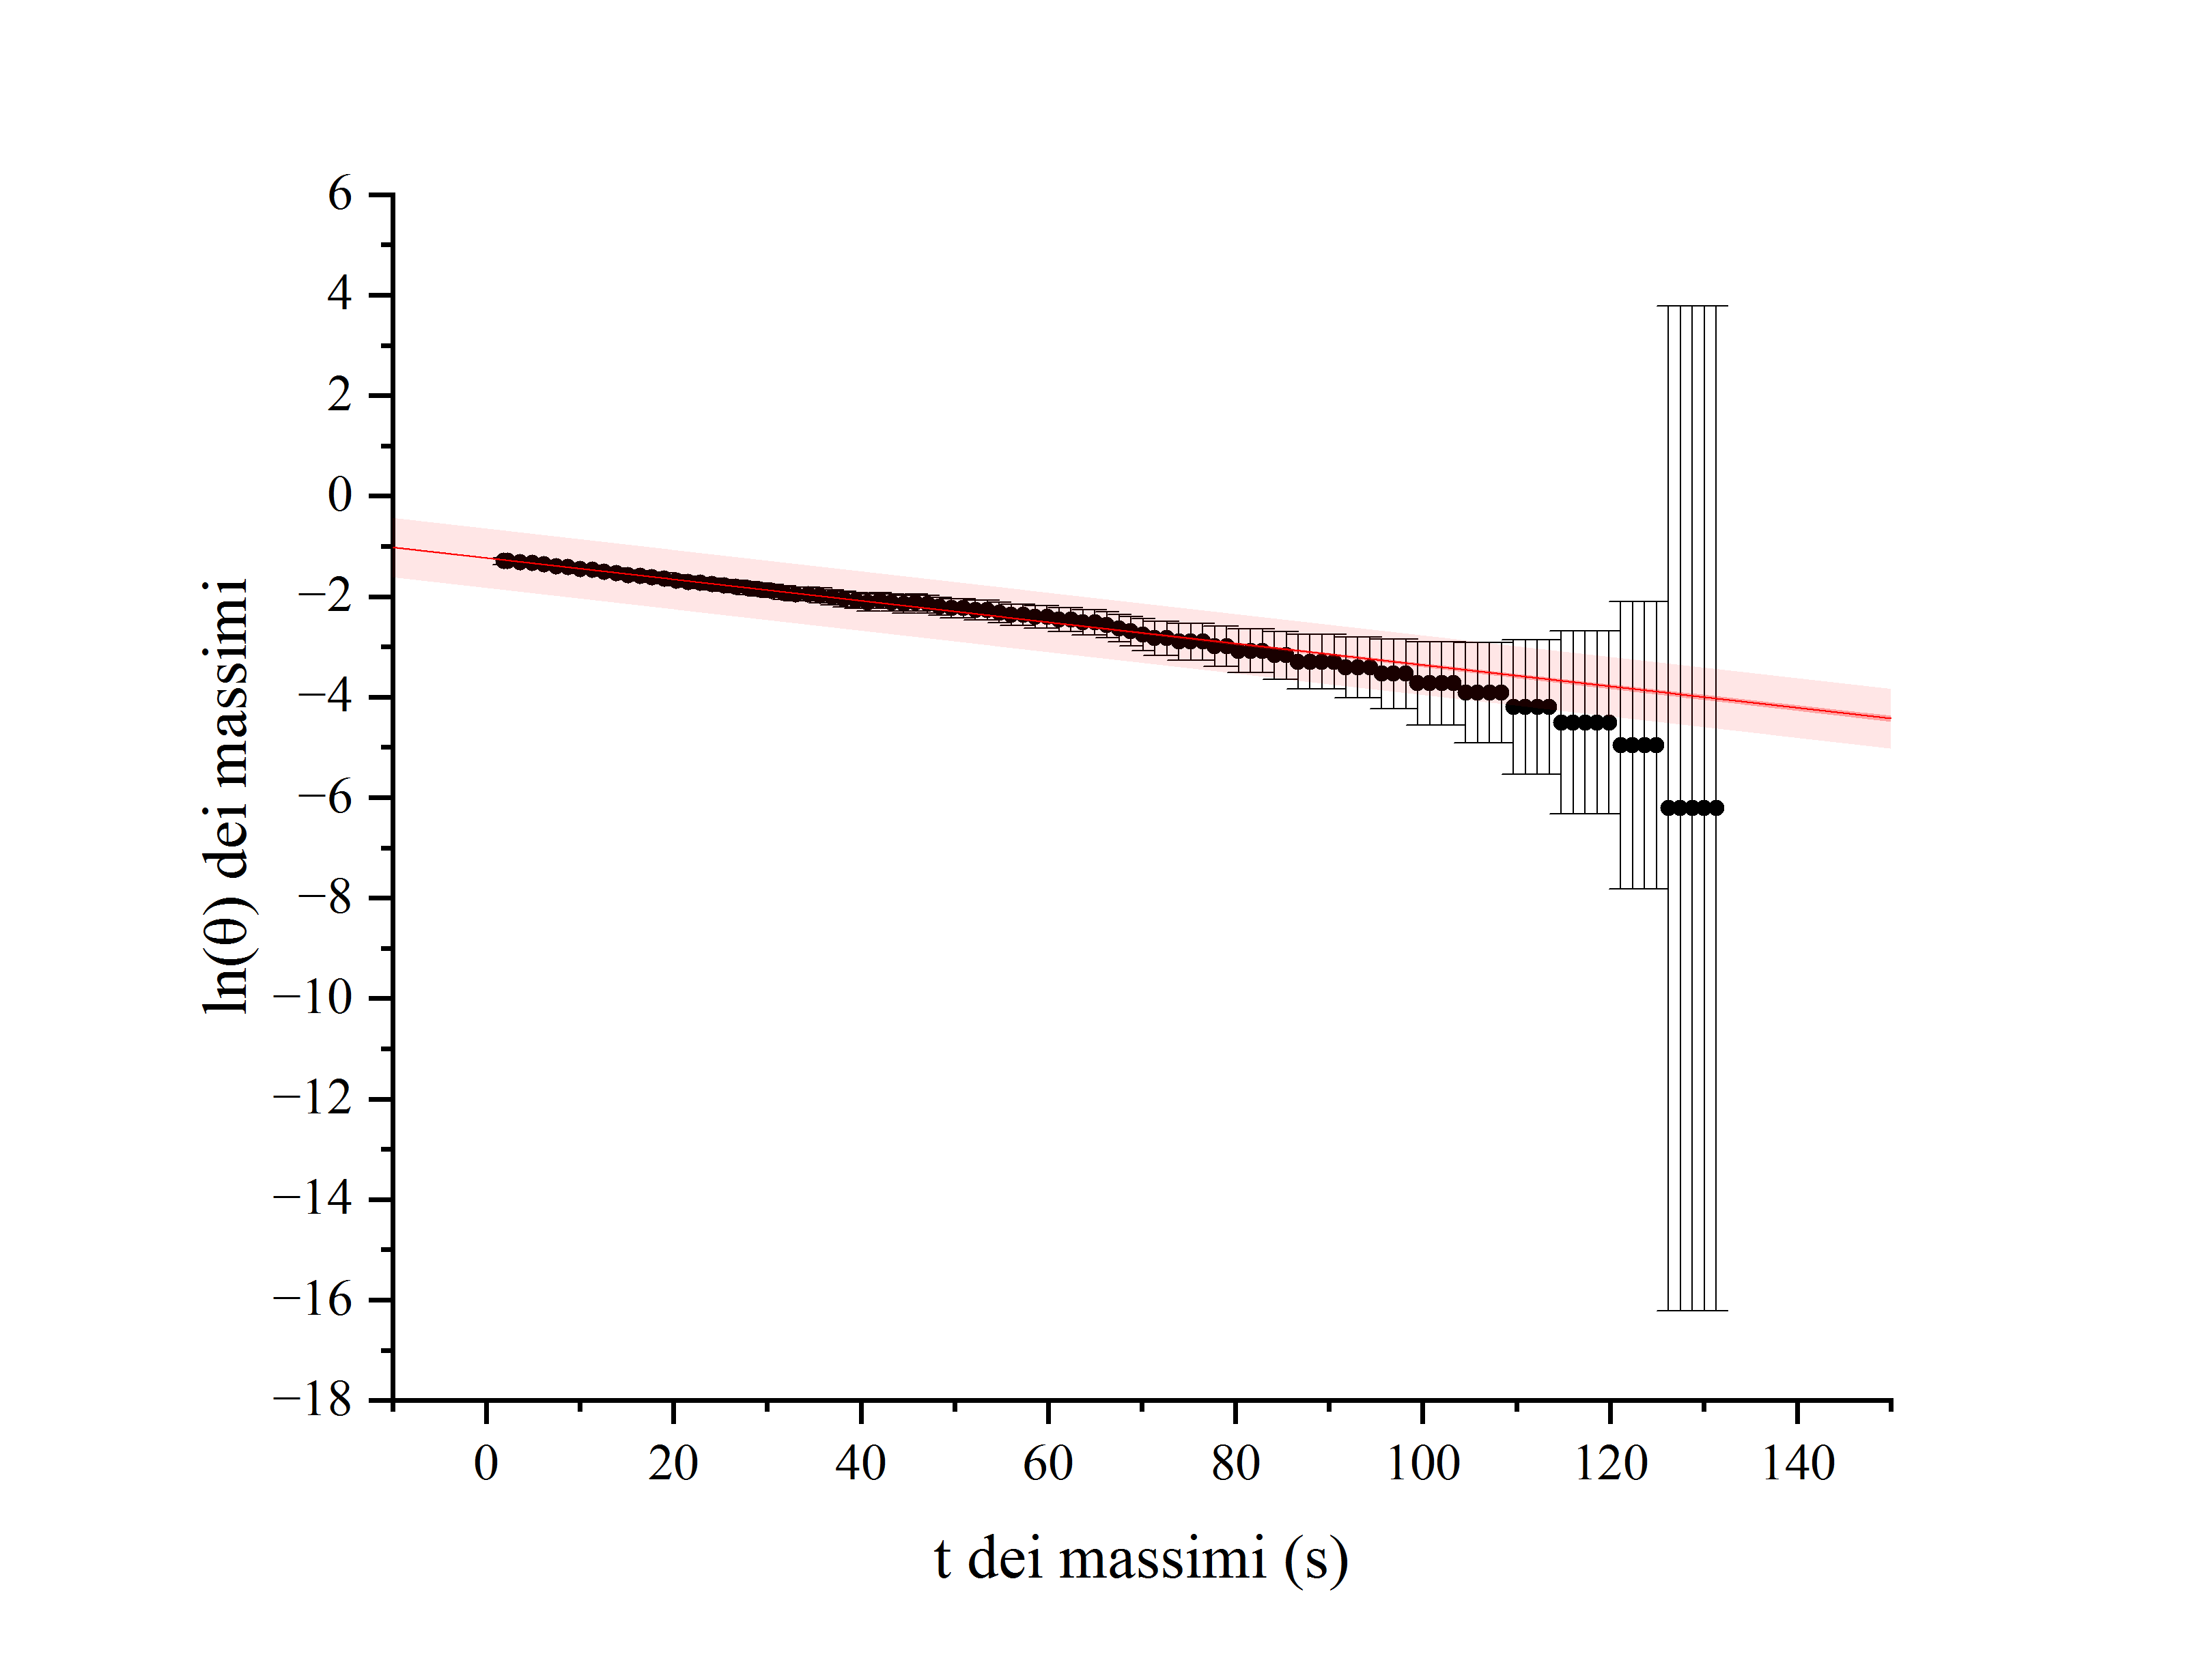
\includegraphics[trim={2cm 1cm 2cm 2.1cm},clip,width=.5\textwidth]{img/0max-exp.png}
    %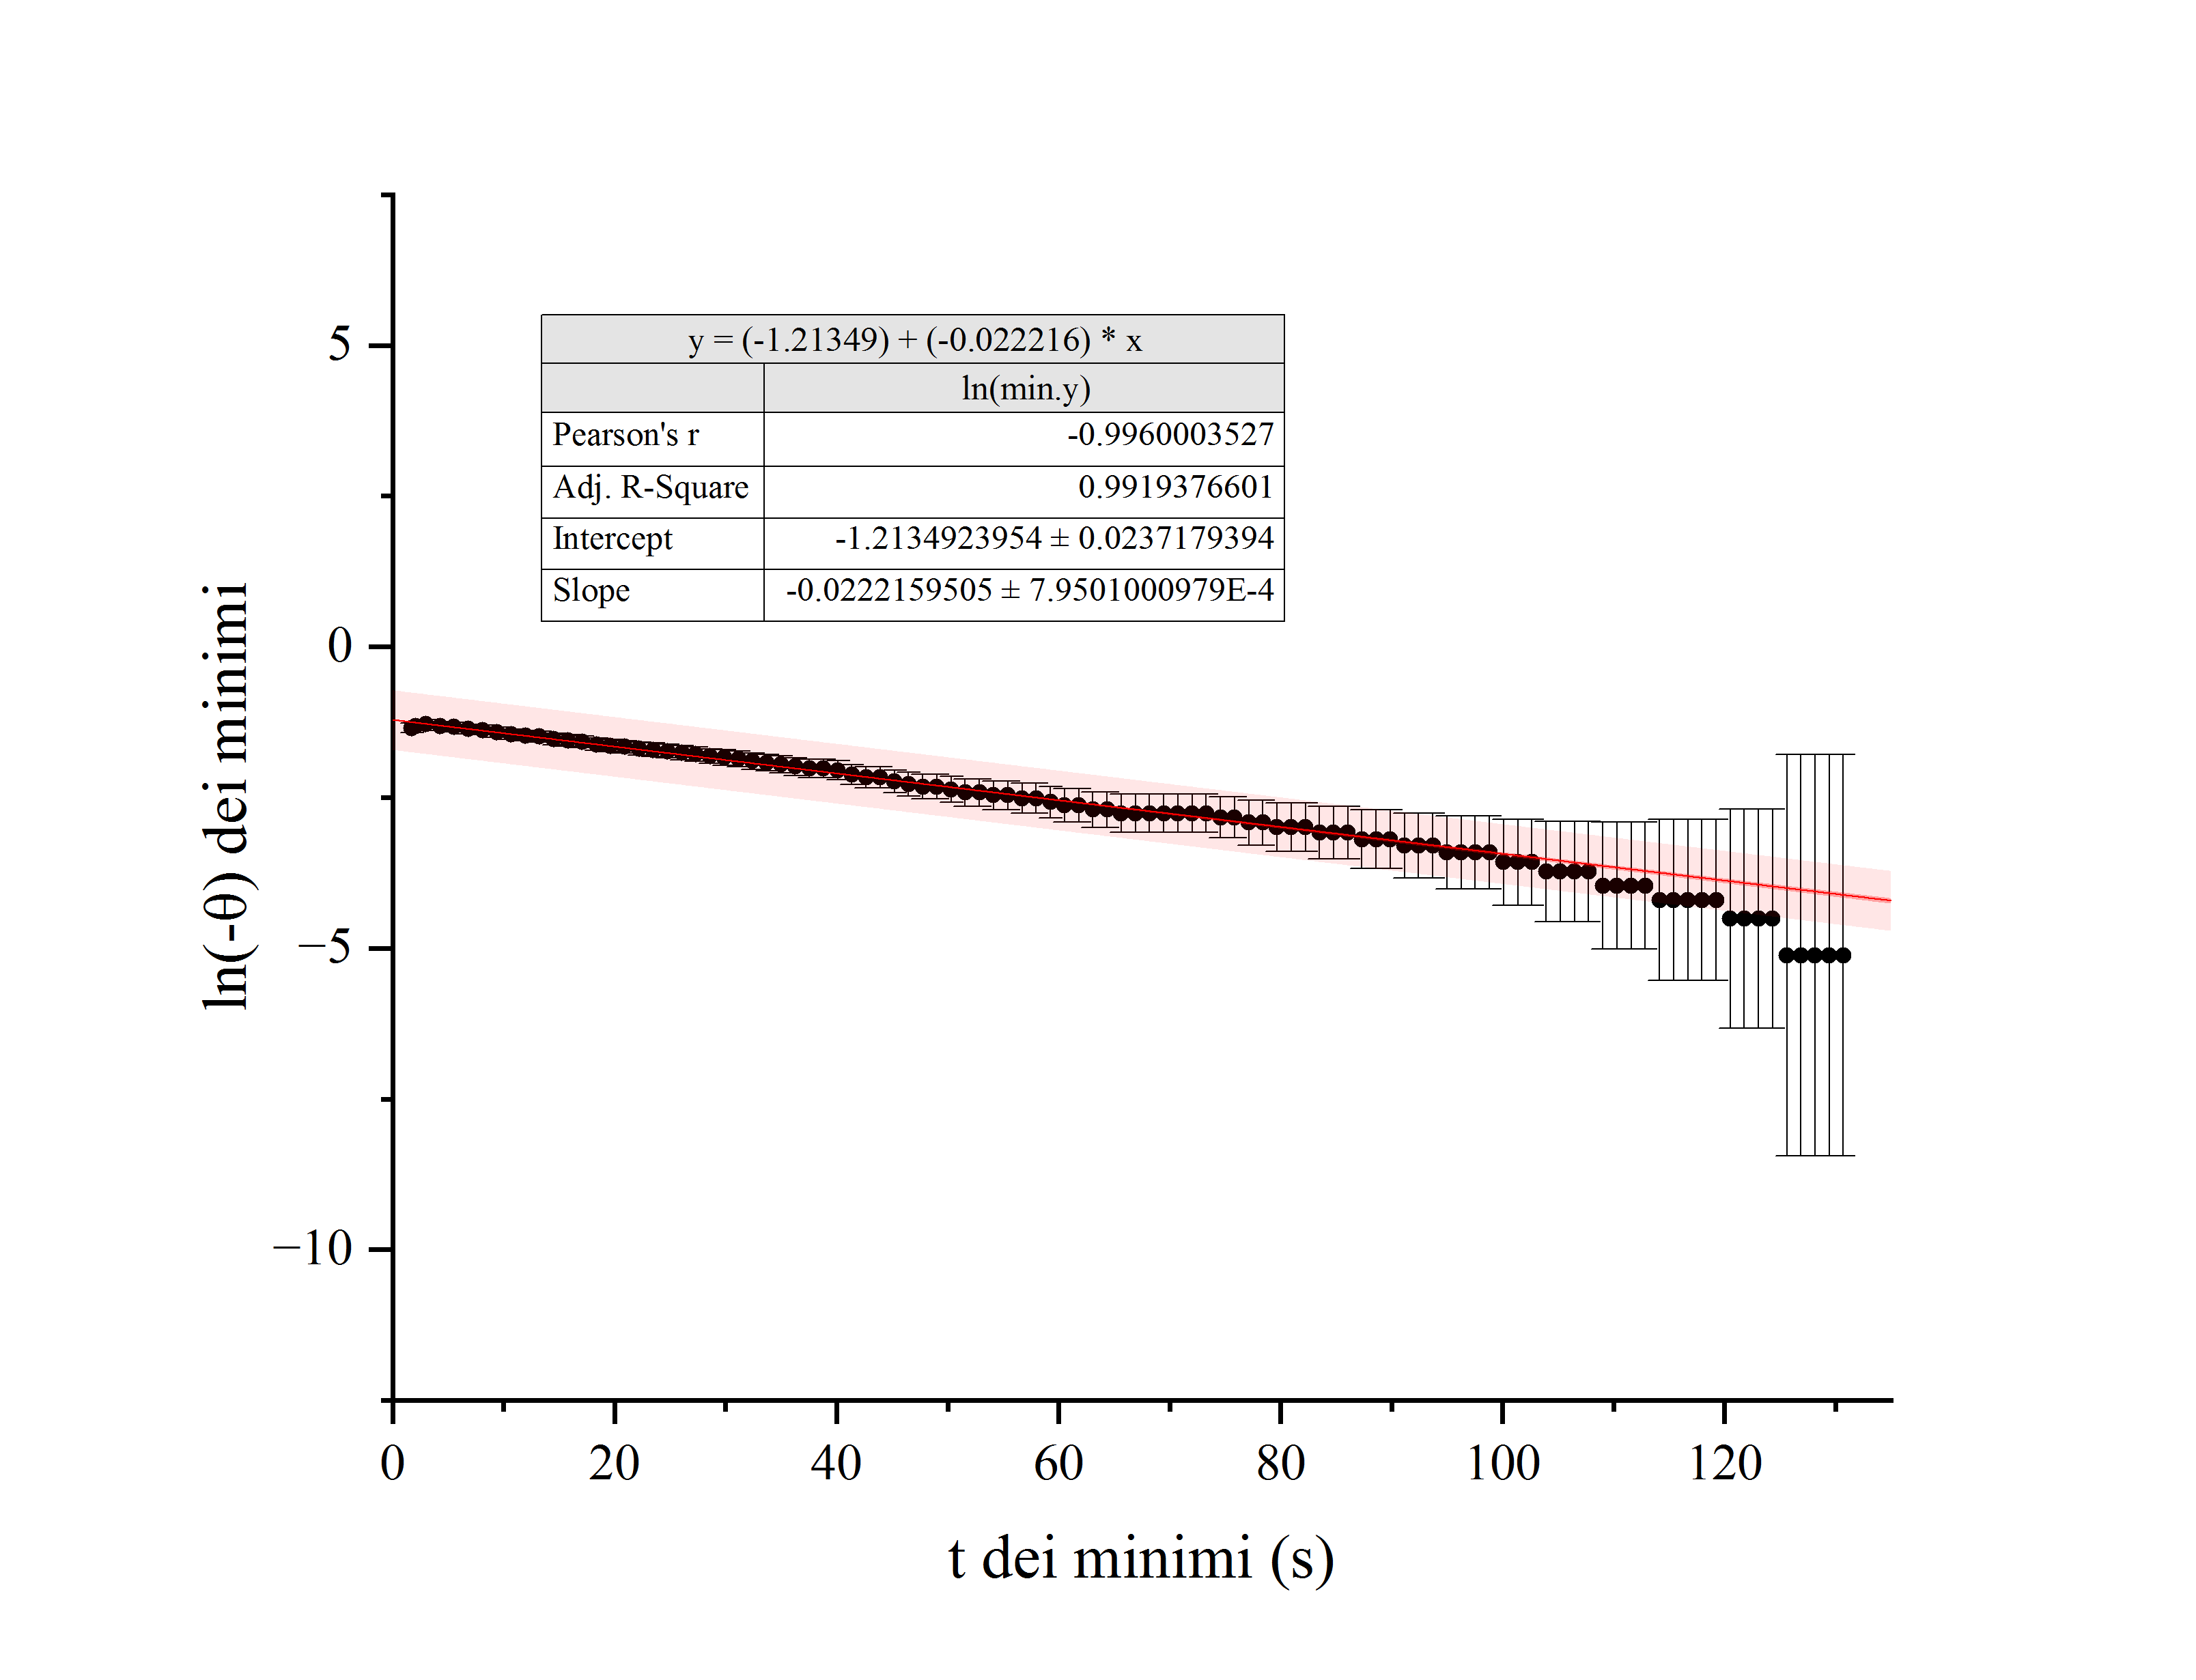
\includegraphics[trim={2cm 1cm 2cm 2.1cm},clip,width=.5\textwidth]{img/0min-exp.png}
    \caption[]{\emph{
      $\ln\left|\theta(t)\right|$ di massimi e minimi,
      su scala logaritmica (per $\Gamma=\left\{\right\}$).
      Sono riportate anche le barre di errore sull'ordinata.
      In rosso, la retta di regressione lineare
      e in rosa la sua regione di incertezza.
    }}
  \end{figure}
\end{center}

Poiché l'obiettivo è calcolare $g$, la correzione da effettuare
sul periodo, per tenere conto dell'attrito, è la seguente:
\[
  T_0^2 = \frac{4\pi^2}{\omega_0^2}
    = \frac{4\pi^2}{\omega^2 + \lambda^2}
    = \frac{4\pi^2}{\frac{4\pi^2}{T^2} + \lambda^2}
    = \frac{1}{\frac{1}{T^2} + \frac{\lambda^2}{4\pi^2}}
\]

Effettuata questa correzione per ogni configurazione $\Gamma$,
si può allora costruire nuovamente una retta di regressione,
analogamente a quanto fatto nella sezione precedente.
La relazione fra le grandezze misurate, ricordiamo, è lineare:
\[ \frac{I_z^\text{\,tot}}{Mr_\text{CM}} = g \frac{T_0^2}{4\pi^2} \]

Riportiamo di seguito il grafico della nuova regressione,
unitamente ai risultati ottenuti.

\begin{figure}[H]
  %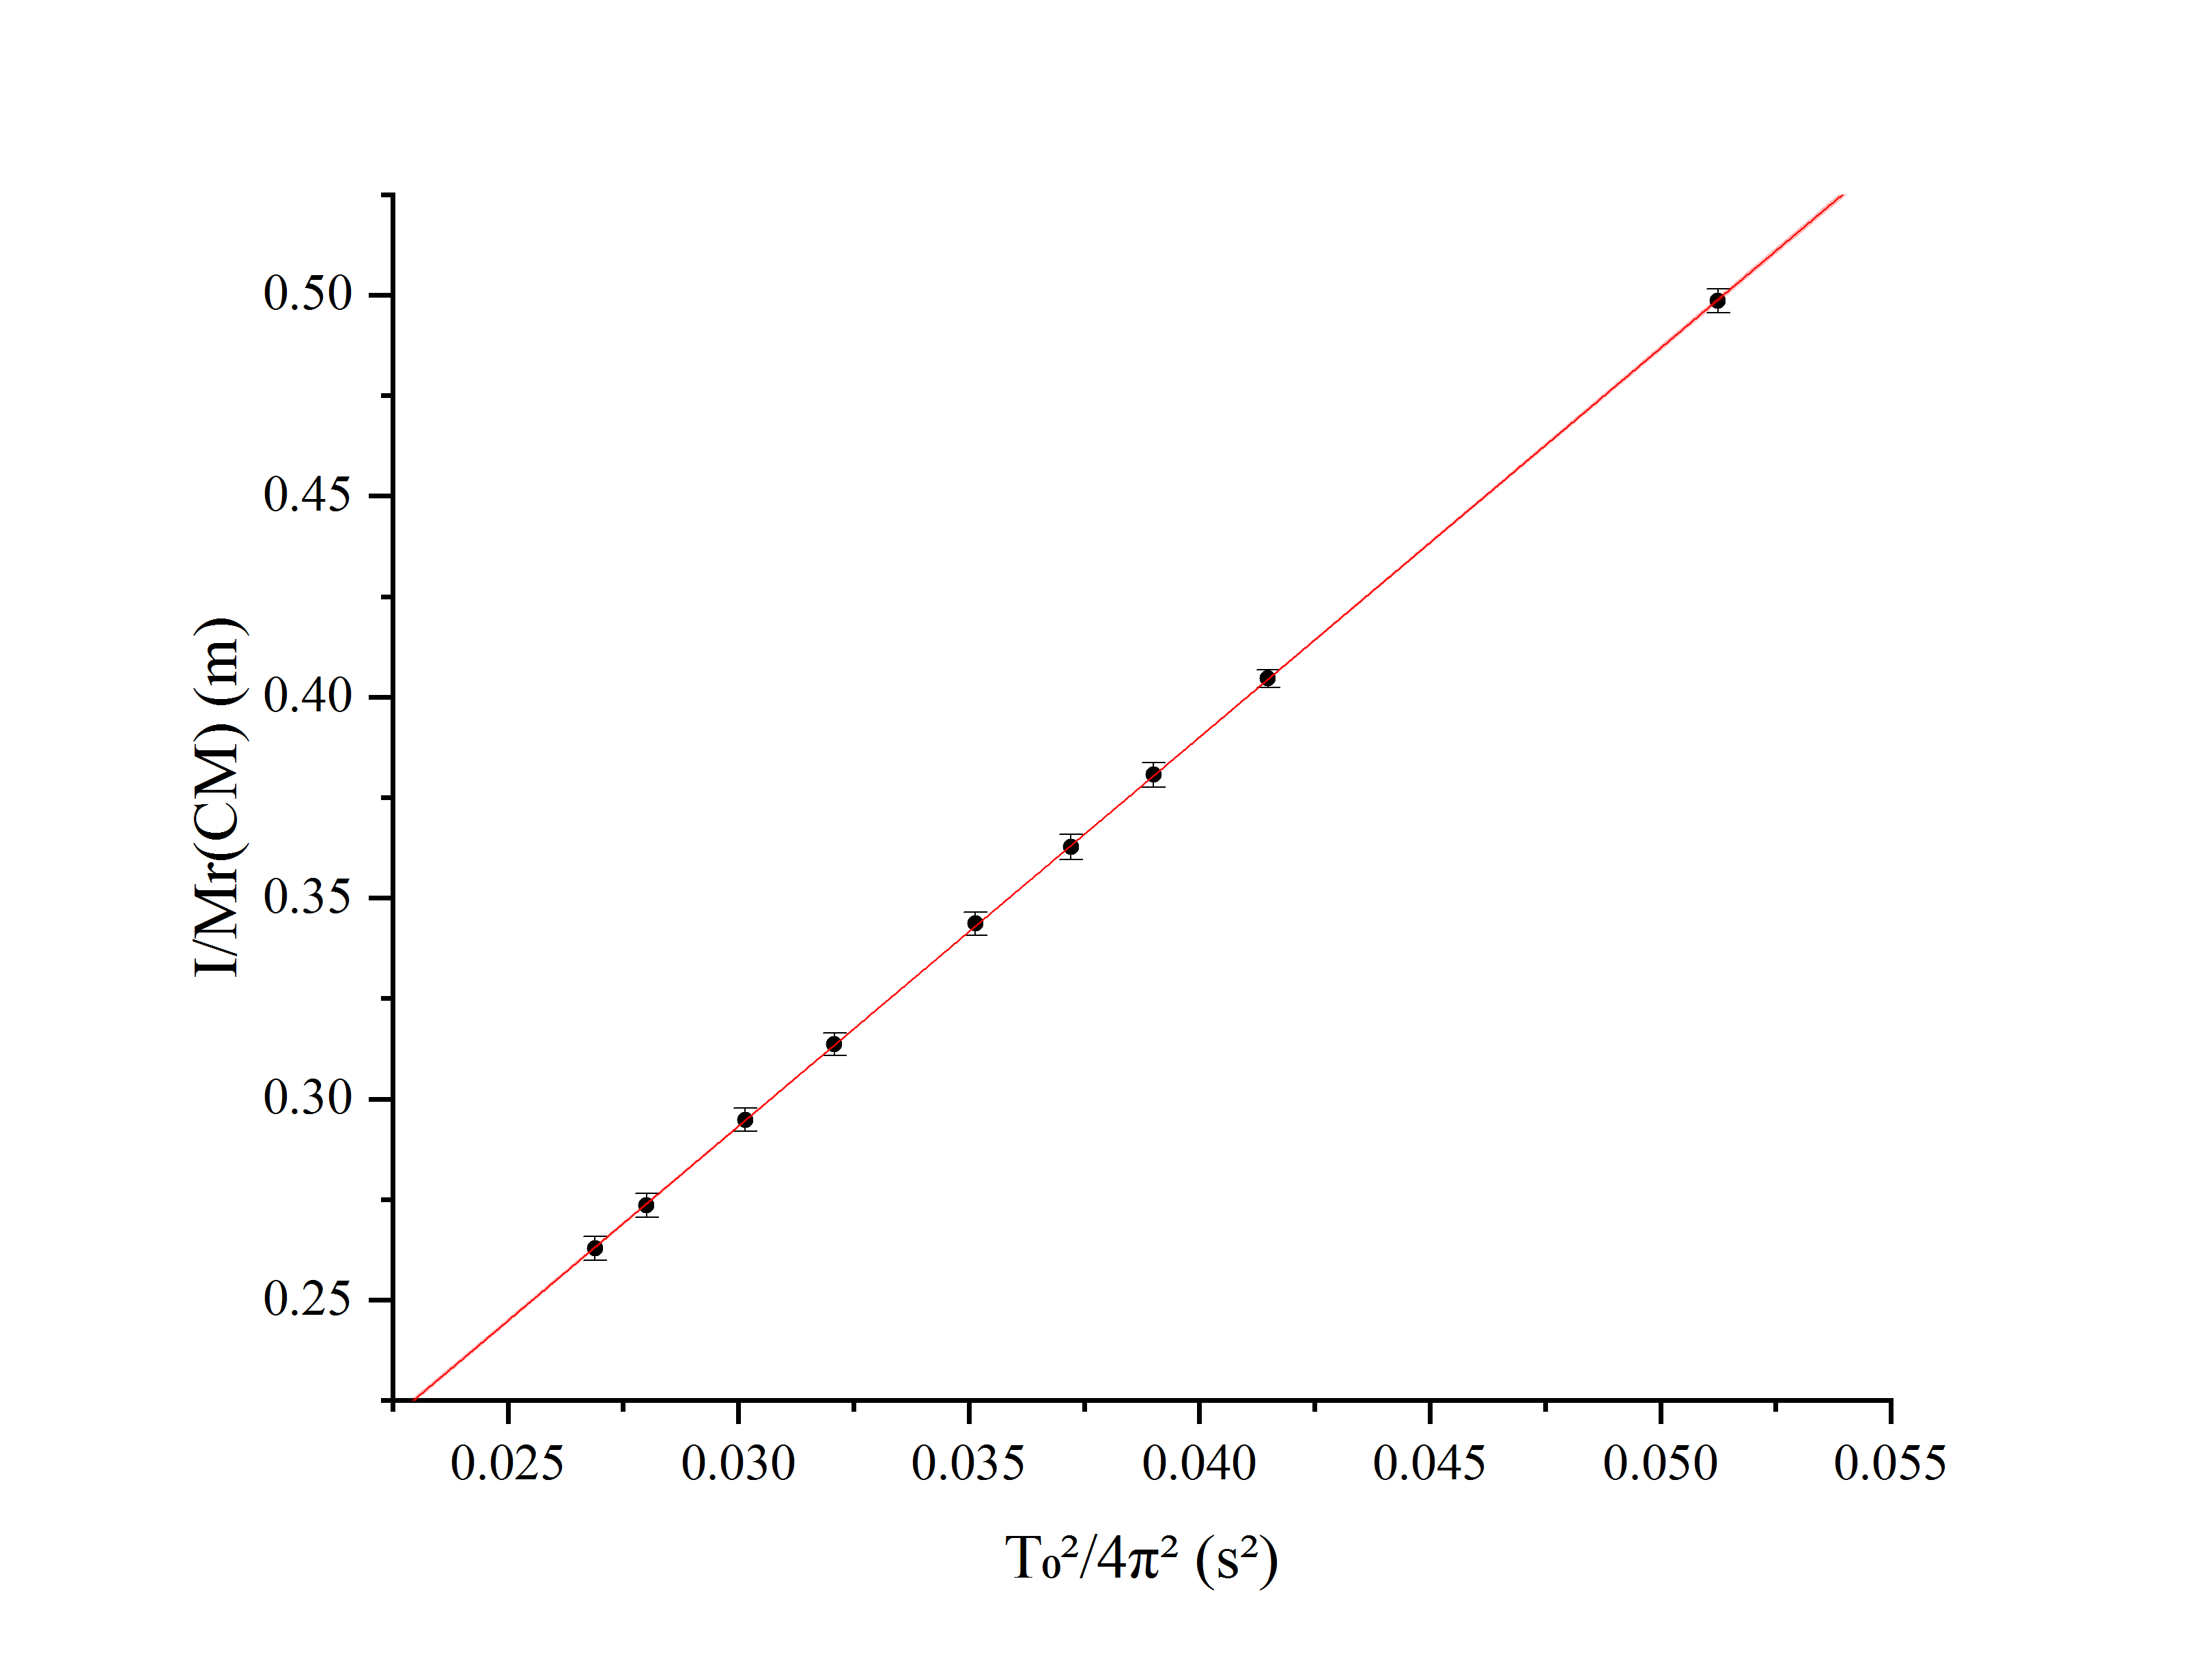
\includegraphics[trim={2cm 1cm 2cm 2.1cm},clip,width=\textwidth]{img/regressione-2.png}
  \caption[]{\emph{
    In rosso, la retta di regressione lineare e in rosa,
    appena visibile, la sua regione di incertezza.
    (le barre di errore sull'ascissa sono così ridotte
    da risultare invisibili)
  }}
\end{figure}

I risultati della regressione lineare sono i seguenti:
\begin{itemize}
  \item Intercetta $= (0.003 \pm 0.005)\;\unit{m}$
  \item Coefficiente angolare $g = (9.68 \pm 0.13)\;\unit{m\per s^2}$
\end{itemize}

Come è possibile osservare comparando questi risultati a
quelli precedentemente ottenuti, il valore di $g$ risultante
è rimasto essenzialmente invariato (al netto della sua incertezza).

In conclusione, possiamo affermare ragionevolmente che,
rispetto alla sensibilità degli strumenti di misura,
il contributo dell'attrito è trascurabile.

\end{document}
